
%%% Local Variables:
%%% mode: latex
%%% TeX-master: t
%%% End:

\documentclass{standalone}
\usepackage{tikz}
\usepackage{amsmath}
\usepackage{pgfplots}
\usepackage{inconsolata}
\usetikzlibrary{shapes.arrows,matrix,arrows,calc,fadings,decorations.pathreplacing,positioning}

 \renewcommand{\familydefault}{\sfdefault}
\begin{document}
\pagestyle{empty}

\def\xmargin{0.1}
\def\ymargin{0.1}
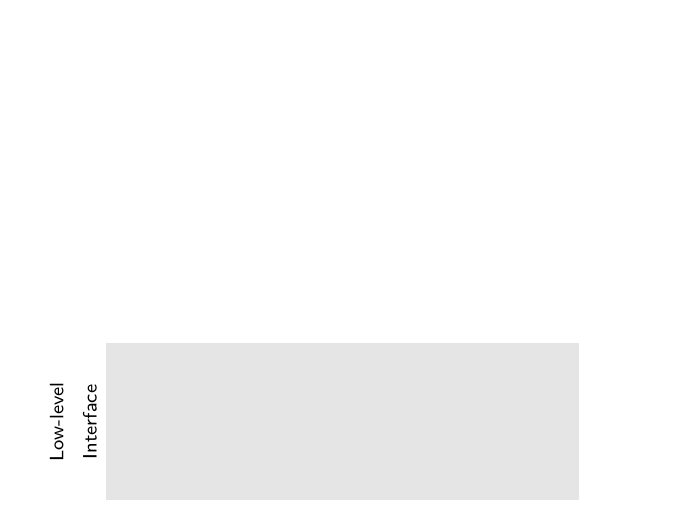
\begin{tikzpicture}[shorten >=1pt,->,draw=black!50, node distance=\layersep]
\clip (-1,6) rectangle (7,0);

    \tikzstyle{backend}=[draw=none];
%   \node [fill=black!20, single arrow, rotate = 270]  at (2,5) {\tiny{\texttt{ TrainGPU(...)}}};
%   \node [fill=black!20, single arrow, rotate = 270]  at (4,5) {\tiny{\texttt{ TrainCPU(...)}}};

% \node[anchor=south, rotate=90, xshift=0.2,text width=2cm] at (0,3.2) {\scriptsize{ OO Model}};
% \fill[black!0] (0,2) rectangle (6,4);
% \draw (\xmargin,2 + \ymargin) rectangle (6-\xmargin,4-\ymargin);
% \draw (2*\xmargin,2 + 2*\ymargin) rectangle (2-\xmargin,3 - \ymargin)
%       node[pos=.5] {\scriptsize \texttt{TBatch}};
% \draw (2*\xmargin,3 + \ymargin) rectangle (2-\xmargin,4 - 2* \ymargin)
%       node[pos=.5] {\scriptsize \texttt{TDataLoader}};
% \draw (2+\xmargin,2 + 2*\ymargin) rectangle (6-2*\xmargin,3 - \ymargin)
%       node[pos=.5] {\scriptsize \texttt{TLayer}};
% \draw (2+\xmargin,3 + \ymargin) rectangle (6-2*\xmargin,4 - 2* \ymargin)
%       node[pos=.5] {\scriptsize \texttt{TNet}};


\node[anchor=south, rotate=90, xshift=-0.2, align=center, text width=2cm] at (0,1) {\scriptsize{Low-level\\ Interface}};
% Cuda

 \fill[black!10] (0,0) rectangle (6,2);

% \draw[fill=violet!20, draw=none] (\xmargin,\ymargin) rectangle (2-\xmargin,2-\ymargin);
% \node[anchor=north, yshift=-0.1cm]  at (1,2) {\small\texttt{TCuda}};
% \draw[fill=violet!40, draw=none] (2*\xmargin,0.9) rectangle (2-2*\xmargin,1.45)
%       node[pos=.5] {\scriptsize \texttt{TCudaMatrix}};
% \draw[fill=violet!40, draw=none] (2*\xmargin,2*\ymargin)
%      rectangle (1-\xmargin,0.9-\ymargin)
%       node[pos=.5] {\tiny \texttt{cuBLAS}};
% \draw[fill=violet!40, draw=none](1+\xmargin,2*\ymargin) rectangle (2-2*\xmargin,0.9-\ymargin)
%       node[pos=.5] {\tiny \texttt{curand}};

% %CPU
% \draw[fill=violet!20, draw=none] (2 + \xmargin,\ymargin) rectangle (4-\xmargin,2-\ymargin);
% \node[anchor=north, yshift=-0.1cm]  at (3,2) {\small\texttt{TCpu}};
% \draw[fill=violet!40, draw=none] (2 + 2*\xmargin,0.9) rectangle (4-2*\xmargin,1.45)
%       node[pos=.5] {\scriptsize \texttt{TCpuMatrix}};
% \draw[fill=violet!40, draw=none] (2 + 2*\xmargin,2*\ymargin)
% rectangle (3-\xmargin,0.9-\ymargin)
%       node[pos=.5] {\tiny \texttt{BLAS}};
% \draw[fill=violet!40, draw=none] (3 + \xmargin,2*\ymargin)
%  rectangle (4-2*\xmargin,0.9-\ymargin)
%       node[pos=.5] {\tiny \texttt{TBB}};

% % OpenCL
% \draw[fill=black!10, draw=none] (4 + \xmargin,\ymargin) rectangle (6-\xmargin,2-\ymargin);
% \node[anchor=north, yshift=-0.1cm]  at (5,2) {\small\texttt{TOpenCL}};
% \draw[fill=black!30, draw=none] (4 + 2*\xmargin,0.9) rectangle (6-2*\xmargin,1.45)
%       node[pos=.5] {\scriptsize \texttt{TCpuMatrix}};
% \draw[fill=black!30, draw=none] (4 + 2*\xmargin,2*\ymargin) rectangle (5-\xmargin,0.9-\ymargin)
%       node[pos=.5] {\tiny \texttt{BLAS}};
% \draw[fill=black!30, draw=none] (5 + \xmargin,2*\ymargin) rectangle (6-2*\xmargin,0.9-\ymargin)
%       node[pos=.5] {\tiny \texttt{TBB}};
\end{tikzpicture}
% End of code
\end{document}
%%% Local Variables:
%%% mode: latex
%%% TeX-master: t
%%% End:
